\documentclass[10pt]{article}
\usepackage{amsmath, amssymb, amsthm}
\usepackage{geometry}
\geometry{a4paper, margin=1in}

\usepackage{lmodern}
\usepackage{parskip}
\usepackage{enumitem}
\usepackage{hyperref}
\usepackage{multicol}
\usepackage{xcolor}
\usepackage{fancyhdr}
\usepackage{graphicx}
\usepackage{amsmath, amssymb, amsthm}
\usepackage{tikz}

\definecolor{mypink}{RGB}{255, 105, 180}
\definecolor{mydarkpink}{RGB}{199, 21, 133}
\definecolor{mygray}{RGB}{80, 80, 80}
\hypersetup{
    colorlinks=true,
    linkcolor=mydarkpink,
    urlcolor=mydarkpink,
    citecolor=mydarkpink
}


\def\HS{\hspace{\fontdimen2\font}}

\pagestyle{fancy}
\fancyhf{}
\fancyhead[L]{\textcolor{mygray}{Elijah's Math Notes}}
\fancyhead[R]{\textcolor{mygray}{\thepage}}
\fancyfoot[C]{\textcolor{mygray}{Prepared by Elijah}}

\usepackage{titling}
\pretitle{\begin{center}\Large\color{mypink}}
\posttitle{\par\end{center}\vskip 0.5em}
\preauthor{\begin{center}\large\color{mygray}}
\postauthor{\par\end{center}}
\predate{\begin{center}\small\color{mygray}}
\postdate{\par\end{center}}

\theoremstyle{plain}
\newtheorem{theorem}{Theorem}[section]
\newtheorem{lemma}[theorem]{Lemma}
\newtheorem{proposition}[theorem]{Proposition}
\newtheorem{corollary}[theorem]{Corollary}

\theoremstyle{definition}
\newtheorem{definition}[theorem]{Definition}
\newtheorem{example}[theorem]{Example}

\theoremstyle{remark}
\newtheorem{remark}[theorem]{Remark}
\newtheorem{note}[theorem]{Note}

\newcommand{\R}{\mathbb{R}}
\newcommand{\N}{\mathbb{N}}
\newcommand{\Z}{\mathbb{Z}}
\newcommand{\todo}[1]{\textcolor{mydarkpink}{\textbf{TODO:} #1}}
\newcommand{\highlight}[1]{\textcolor{mypink}{#1}}

\renewcommand{\theenumi}{\Alph{enumi}}

\title{Vermont State Mathematics Coalition Talent Search Test \#2}
\author{Elijah Renner}
\date{\today}

\begin{document}

\maketitle
\tableofcontents

\section{Problem \#1}

\subsection{a}

\paragraph{Problem} A parallelogram has altitudes of lengths \(3\) and \(4\), and its perimeter is \(84\). What is its area?

\paragraph{Solution} Let \(a\) and \(b\) be the sides corresponding to altitudes \(3\) and \(4\), respectively. Since the same area of a parallelogram is given by the product of either side and its corresponding altitude, \(3a=4b\). And, since we know that the perimeter is \(84\), it follows that \(2a+2b=2(a+b)=84\). Solving this system for \(a\) and \(b\), \((a,b)= (24,18)\). Then, multiplying either \(a\) or \(b\) by its corresponding altitude, \[A_{\text{parallelogram}}=3a=4b=3(24)=4(18)=\fbox{72}\]

\subsection{b}

\paragraph{Problem} Let \(A\) be the answer to part \((a)\). The sum of the terms in an infinite geometric sequence equals \(1\) and the sum of the squares of the terms in the sequence equals \(\frac{1}{A}\). What is the first term of the sequence?

\paragraph{Solution} Since the terms in the sequence have a sum of \(1\), the common ratio \(r\) must have the property \(|r|<1\). The sum to infinite terms in a convergent sequence is given by \(\frac{a}{1-r}\) where \(a\) is the first term of the sequence\footnote{Since the general formula \(\frac{a(1-r^\infty)}{1-r}\) for the sum of \(n\) terms of a geometric sequence, convergent or non-convergent, becomes \(\frac{a(1-0)}{1-r}\) for \(|r|<1\) (a property of convergent geometric sequences).}. So, the sum of terms in the sequence \(S=\frac{a}{1-r}=1\implies a=1-r\). 

Next, given \(A=72\), the sum of the squares of the terms in the sequence is \(\hat{S} = \frac{1}{A} = \frac{1}{72}\). We can deduce\footnote{Consider a geometric sequence with first term \(a\) and common ratio \(r\): \((a, ar, ar^2, ar^3, \dots)\). Squaring all terms, the sequence becomes \((a^2, (ar)^2, (ar^2)^2, (ar^3)^2, \dots)\). The sum of the squared terms then becomes \(a^2 + (ar)^2 + (ar^2)^2 + \dots = a^2(1 + r^2 + r^4 + r^6 + \dots).\)
The series \(1 + r^2 + r^4 + r^6 + \dots\) is a geometric sequence with sum \(\frac{1}{1 - r^2} \quad \text{(valid for } |r| < 1\text{)}.\)
Multiplying by \(a^2\), the sum of all squared terms is \(\frac{a^2}{1 - r^2}\).} that the sum of all terms squared in a convergent geometric sequence is \(\frac{a^2}{1 - r^2}\). Then, \(\frac{1}{72}=\frac{a^2}{1 - r^2}\). Substituting \(a=1-r\) into \(\frac{a^2}{1 - r^2}=\frac{1}{72}\), \(\frac{(1-r)^2}{1-r^2}=\frac{(1-r)^2}{(1-r)(1+r)}=\frac{1-r}{1+r}=\frac{1}{72}\). Solving for \(r\), \(\frac{1-r}{1+r}=\frac{1}{72}\implies72(1-r)=1+r\implies72-72r=1+r\implies73r=71\implies r=\frac{71}{73}\). Substituting \(r\) into \(a=1-r\), \(a=1-(\frac{71}{73})=\fbox{\(\frac{2}{73}\)}\), the first term in the sequence.


\subsection{c}

\paragraph{Problem} Let \(B\) be the answer to part \((b)\), and let \(k\) be the value of \(\frac{1}{B}\) rounded down to the nearest integer. A sphere of volume \(k\pi\) is inscribed in a cube, which is inscribed in a larger sphere, which is in turn inscribed in a regular tetrahedron. Find the surface area of the tetrahedron.

\paragraph{Solution} If \(B=\frac{2}{73}\), \(\frac{1}{B}=\frac{1}{\left(\frac{2}{73}\right)}=
\frac{73}{2}=36.5\). Rounding down \(\frac{1}{B}\) to the nearest integer, \(36\), \(k=36\). So, the sphere inscribed in the cube has volume \(k\pi=36\pi\). The volume of a sphere is related to its radius by \(V=\frac{4}{3}\pi r^3\). To find \(r_{\text{small sphere}}\), substitute \(36\pi\) as    \(V\): \(36\pi=\frac{4}{3}\pi r_{\text{small sphere}}^3\). With manipulation, \(r_{\text{small sphere}}=3\).

Since the small sphere is inscribed in a cube, the cube will have side length \(s_{\text{cube}}=2r_{\text{small sphere}}=2(3)=6.\) The known relationship between the side length \(s\) of a cube which is inscribed inside a sphere and the sphere's radius \(r\) is \(r=\frac{\sqrt{3}}{2}s\). So, it follows that \(r_{\text{large sphere}}=\frac{\sqrt{3}}{2}s_{\text{cube}}=\frac{\sqrt{3}}{2}(6)=3\sqrt{3}\).

To find \(s_{\text{tetrahedron}}\), the relationship between the radius of a sphere inscribed in a tetrahedron \(r\) and the tetrahedron's side length \(l\), \(l=\frac{12}{\sqrt{6}}r\), can be used: \(s_{\text{tetrahedron}}=\frac{12}{\sqrt{6}}(r_{\text{large sphere}})=\frac{12\cdot3\sqrt{3}}{\sqrt{6}}=18\sqrt{2}\). 

Then, it is known that \(SA_{\text{tetrahedron}}=\sqrt{3}s_{\text{tetrahedron}}^2=\sqrt{3}\left(18\sqrt{2}\right)^2=\fbox{648\sqrt3}\)

\section{Problem \#2}

\paragraph{Problem} In the diagram below, which is not to scale, the large rectangle is divided into 9 smaller rectangles by lines parallel to its sides. The areas of four of the small rectangles are \(2, 4, 6\), and \(24\), as indicated in the diagram. Find the smallest possible area of the large rectangle.\\

\begin{center}
\begin{tabular}{ |c|c|c| } 
 \hline
2 & 4 & \\ 
\hline
6 && \\ 
\hline
&& 24 \\ 
 \hline
\end{tabular}
\end{center}\

\paragraph{Solution} Let the widths of the three vertical stripes be \(x,y,z\) and the heights of the three horizontal stripes be \(a,b,c\). Then, from the given areas,
\[\text{top-left rectangle: }a\cdot x=2\hspace{1cm}\text{top-middle rectangle: }a\cdot y=4\]
\[\text{middle-left rectangle: }b\cdot x=6\hspace{1cm}\text{bottom-right rectangle: }c\cdot z=24\]
manipulating \(ax=2\implies x=\frac{2}{a}\) and \(ay=4\implies y=\frac{4}{a}\), we observe that \(y=2x\). Manipulating \(bx=6\implies b=\frac{6}{x}=\frac{6}{\frac{2}{a}}=3a\). Using the bottom-right rectangle, \(c=\frac{24}{z}\). Now, the area of the large rectangle \(A\) is \((x+y+z)(a+b+c)=\left(x+\left(2x\right)+z\right)\left(a+\left(3a\right)+\left(\frac{24}{z}\right)\right)=(3x+z)(4a+\frac{24}{z})\). Inserting \(x=\frac{2}{a}\), \(A=\left(\frac{6}{a}+z\right)\left(4a+\frac{24}{z}\right)=48+\frac{144}{az}+4az\). With \(A\) in terms of \(az\), we aim to minimize \(A\). By the AM-GM inequality, \(\frac{\frac{144}{az}+4az}{2}\geq\sqrt{\frac{144}{az}\cdot 4az}\implies\frac{\frac{144}{az}+4az}{2}\geq\sqrt{576}\implies\frac{144}{az}+4az\geq 48\). In this case, the minimum of \(\frac{144}{az}+4az\) occurs at equality. We know that equality occurs in the AM-GM inequality for \(\frac{144}{az}=4az\). Solving for \(az\), \(az=\pm6\). We're only concerned with \(+6\), though. Substituting the \(az=6\) that minimizes \(A\), the smallest possible area is \[A=48+\frac{144}{az}+4az=48+\frac{144}{(6)}+4(6)=\fbox{96}\]

\section{Problem \#3}

\paragraph{Problem} Ragulan and Kevin are playing a game with a pile of stones, with Ragulan going first. Each turn, a player may take any prime number of stones, or 1 stone. The player who takes the last stone wins. The players randomly select to play with \(n\) starting stones where \(1\leq n\leq 2024\). For how many \(n\), with \(1\leq n\leq 2024\), does Ragulan have a strategy that guarantees he can win the game?

\paragraph{Solution}First, define a position \(n\) as \textit{losing} if the player about to move has no strategy to force a win, assuming both players play optimally. Conversely, a position is \textit{winning} if the player can force a win from that position. Based on the rules of the game, from a position with \(n\) stones, a player may remove \(1\) stone or any prime number of stones \(p\leq n\). In the base case \(n=1\), the player can take 1 stone and win. Hence, \(n=1\) is a winning position. Gathering more data,
\[ \begin{align*} n=2 &: \text{Take 2 stones to win immediately. Winning.} \\ n=3 &: \text{Take 3 stones to win immediately. Winning.} \\ n=4 &: \begin{cases} \text{Take 1 stone } &\Rightarrow n=3 \text{ (winning for opponent)} \\ \text{Take 2 stones } &\Rightarrow n=2 \text{ (winning for opponent)} \\ \text{Take 3 stones } &\Rightarrow n=1 \text{ (winning for opponent)} \end{cases}  \end{align*} \]
All possible moves for \(n=4\) lead to winning positions for the opponent. Thus, \(n=4\) is a losing position. By further analysis, it becomes apparent that every \(n\) such that \(n\mod 4=0\) is a losing position. All such \(n\) \((\text{e.g., }n=8,12,16,...)\), satisfy that any move from \(n\) yields a non-multiple of 4, i.e., a winning position. Conversely, from any non-multiple of 4, a player can always move to a multiple of 4, forcing the opponent into a losing position. Given this, the number of losing positions is \(\left\lfloor \frac{2024}{4} \right\rfloor = 506\). And, therefore, \[\text{Winning positions}=\text{Total positions}-\text{Losing positions}=2024-506=\fbox{1518}\]

\section{Problem \#4}

\paragraph{Problem} Find all ordered pairs \((a,b)\) of positive integers such that \(\left(\sqrt{a+\sqrt{2024}}+\sqrt{b-\sqrt{2024}}\right)^2\) is a rational number.

\paragraph{Solution}
Let $r=\sqrt{2024}$. We seek positive integers $(a,b)$ such that
\[
\left(\sqrt{a+r}+\sqrt{b-r}\right)^2 = a+b+2\sqrt{(a+r)(b-r)}
\]
is rational. For this to hold, $\sqrt{(a+r)(b-r)}$ must be rational. Therefore, we write $(a+r)(b-r)=q^2$ for some rational $q$. Expanding:
\[
(a+r)(b-r)=ab - 2024 + \sqrt{2024}(b - a).
\]
Since $\sqrt{2024}$ is irrational, the term involving it must vanish for the product to be a rational square. Thus $b=a$. Substituting back, we get:
\[
(a+r)(a-r) = a^2 - 2024 = q^2.
\]
Set \(a^2 - q^2 = 2024\), which factors as (a - q)(a + q) = 2024.
To find integer solutions, consider the four factor pairs \((d_1=[a-q], d_2=[a+q])\) of 2024 where \(d_1 < d_2\):
\[
(2, 1012),\ (4, 506),\ (22, 92),\ (44, 46)
\]
For each pair, solve for \(a\) and \(q\):
\[
a = \frac{d_1 + d_2}{2}, \quad q = \frac{d_2 - d_1}{2}
\]
Calculations yield:
\begin{align*}
(2, 1012): &\quad a = 507,\ q = 505 \\
(4, 506): &\quad a = 255,\ q = 251 \\
(22, 92): &\quad a = 57,\ q = 35 \\
(44, 46): &\quad a = 45,\ q = 1
\end{align*}
Then, using \(a=b\) for all determined \(a\), the solutions are
\[
\fbox{\((a,b)\in\{\,(45,45),\ (57,57),\ (255,255),\ (507,507) \,\}\)}
\]

\section{Problem \#5}

\paragraph{Problem} Find all the angles \(\theta \in[0,\pi]\) such that \(\sin(5\theta)=8\sin(\theta-\frac{\pi}{5})\sin(\theta+\frac{\pi}{5})\sin(\theta-\frac{2\pi}{5})\sin(\theta+\frac{2\pi}{5})\).

\paragraph{Solution} To solve the equation 
\[
\sin(5\theta) = 8\sin\left(\theta-\frac{\pi}{5}\right)\sin\left(\theta+\frac{\pi}{5}\right)\sin\left(\theta-\frac{2\pi}{5}\right)\sin\left(\theta+\frac{2\pi}{5}\right)
\]
for \(\theta \in [0, \pi]\), we first find values \(\theta\) for the case where \(\sin(5\theta) = 0\). This occurs at \(\theta = \frac{k\pi}{5}\) for \(k = 0, 1, 2, 3, 4, 5\). Substituting these values, we find that \(\theta = 0\) and \(\theta = \pi\) do not satisfy the original equation since the rhs does not disappear. However, \(\theta = \frac{\pi}{5}, \frac{2\pi}{5}, \frac{3\pi}{5}, \frac{4\pi}{5}\) are valid solutions as the rhs becomes zero due to one of the sine factors being zero.

Next, we explore solutions where \(\sin(5\theta) \neq 0\). By testing common angles, we substitute \(\theta = \frac{\pi}{6}\) and \(\theta = \frac{5\pi}{6}\) into both sides of the equation:
\[
\sin\left(5 \cdot \frac{\pi}{6}\right) = \sin\left(\frac{5\pi}{6}\right) = \frac{1}{2},
\]
and evaluating the RHS at \(\theta = \frac{\pi}{6}\) also yields \(\frac{1}{2}\). Similarly, for \(\theta = \frac{5\pi}{6}\),
\[
\sin\left(5 \cdot \frac{5\pi}{6}\right) = \sin\left(\frac{25\pi}{6}\right) = \sin\left(\frac{\pi}{6}\right) = \frac{1}{2},
\]
and the RHS similarly evaluates to \(\frac{1}{2}\). Thus, these angles satisfy the equation.

Combining both cases, the complete set of solutions in \([0, \pi]\) is:
\[
\boxed{\frac{\pi}{5},\ \frac{2\pi}{5},\ \frac{3\pi}{5},\ \frac{4\pi}{5},\ \frac{\pi}{6},\ \frac{5\pi}{6}}.

\section{Problem \#6}

\paragraph{Problem} For a positive integer \(n\), define \(g(n)\) to be the number of positive integers less than or equal to \(n\) whose prime divisors all lie in the set \(\{2,3\}\): for example, \(g(10)=7\) and \(g(100)=20\). Prove that there exists a positive constant \(C\) such that \(|g(n)-\frac{1}{2}(\log_2n)(\log_3n)|<C\log_6n\) for all integers \(n\geq 2\).

\paragraph{Proof} Let \( S = \{2^a 3^b : a, b \in \mathbb{Z}_{\geq 0}\} \) be the set of integers whose prime divisors are in \(\{2, 3\}\). Then \( g(n) \) counts the number of elements of \( S \) that do not exceed \( n \). Rewriting the inequality \( 2^a 3^b \leq n \) in logarithmic form, we obtain \(a \ln 2 + b \ln 3 \leq \ln n\), which geometrically describes a triangular region \( R_n \) in the \((a, b)\)-plane, bounded by the coordinate axes and the line \( a \ln 2 + b \ln 3 = \ln n \). The vertices of \( R_n \) are:
\[
(0, 0), \quad \left( \frac{\ln n}{\ln 2}, 0 \right), \quad \text{and} \quad \left( 0, \frac{\ln n}{\ln 3} \right).
\]
\begin{center}
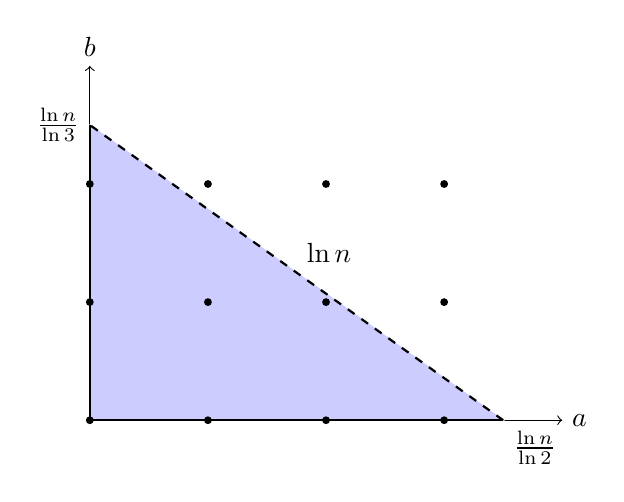
\begin{tikzpicture}[scale=1.5]
  \draw[->] (0,0) -- (4,0) node[right] {\(a\)};
  \draw[->] (0,0) -- (0,3) node[above] {\(b\)};
  \filldraw[blue!20] (0,0) -- (3.5,0) -- (0,2.5) -- cycle;
  \draw[thick] (0,0) -- (3.5,0) node[below right] {\(\frac{\ln n}{\ln 2}\)};
  \draw[thick] (0,0) -- (0,2.5) node[left] {\(\frac{\ln n}{\ln 3}\)};
  \draw[thick, dashed] (3.5,0) -- (0,2.5) node[midway, above right] {\(\ln n\)};
  \foreach \x in {0,1,2,3} {
    \foreach \y in {0,1,2} {
      \node[circle,fill,inner sep=1pt] at (\x,\y) {};
    }
  }
\end{tikzpicture}
\end{center}
The area \( A(R_n) \) of this triangle is \(A(R_n) = \frac{1}{2} \cdot \frac{\ln n}{\ln 2} \cdot \frac{\ln n}{\ln 3} = \frac{1}{2} (\log_2 n)(\log_3 n).\)
Since \( g(n) \) corresponds to the number of lattice points \( (a, b) \) with \( a, b \in \mathbb{Z}_{\geq 0} \) inside \( R_n \), we refine the estimate for \( g(n) \) using standard lattice point results. I.e., for a convex region \( R \) with smooth boundary, the number of lattice points \( N(R) \) satisfies
\[
N(R) = A(R) + \mathcal{O}(P(R)),
\]
where \( A(R) \) is the area of \( R \), and \( P(R) \) is its perimeter. The perimeter \( P(R_n) \) of the triangle is the sum of:
- The base \( \frac{\ln n}{\ln 2} \),
- The height \( \frac{\ln n}{\ln 3} \),
- The hypotenuse, whose length is proportional to \( \ln n \). Thus, \( P(R_n) = \mathcal{O}(\ln n) \).
Substituting into the lattice point estimate, we obtain
\[
g(n) = A(R_n) + \mathcal{O}(P(R_n)) = \frac{1}{2} (\log_2 n)(\log_3 n) + \mathcal{O}(\ln n).
\]
We further simplify the error term \( \mathcal{O}(\ln n) \) using the change of base formula for logarithms \( \ln n = (\ln 6)(\log_6 n) \), giving:
\[
g(n) = \frac{1}{2} (\log_2 n)(\log_3 n) + \mathcal{O}(\log_6 n).
\]
Thus, the inequality
\[
\left| g(n) - \frac{1}{2} (\log_2 n)(\log_3 n) \right| < C \log_6 n
\]
holds for some positive constant \( C \), since the error term \( \mathcal{O}(\log_6 n) \) arises from the perimeter \( P(R_n) \), which is proportional to \( \ln n \).

For further intuition, we may substitute the approximation 
\[
g(n) \approx \frac{1}{2} (\log_2 n)(\log_3 n) + \mathcal{O}(\log_6 n)
\]
into the inequality, where we'll see that
\[
\left| \left( \frac{1}{2} (\log_2 n)(\log_3 n) + \mathcal{O}(\log_6 n) \right) - \frac{1}{2} (\log_2 n)(\log_3 n) \right| = \left| \mathcal{O}(\log_6 n) \right| \implies\left| \mathcal{O}(\log_6 n) \right| < C \log_6 n.
\]
Then, since \( \mathcal{O}(\log_6 n) \) is bounded above by some constant multiple of \( \log_6 n \), clearly there exists a constant \( C > 0 \) such that
\[
\left| g(n) - \frac{1}{2} (\log_2 n)(\log_3 n) \right| < C \log_6 n . \text{ }\square
\]

\end{document}

